
\documentclass[10pt, a4paper]{article}

\usepackage[top=1in, bottom=1in, left=1in, right=1in]{geometry}
%\usepackage{setspace}
%\onehalfspacing
\usepackage{graphicx}
\usepackage{float}

\usepackage{subfig}
\usepackage{amsmath}

\usepackage{amssymb}
\usepackage{fancyhdr}
\usepackage[version=3]{mhchem}
\pagestyle{fancyplain}

\renewcommand{\arraystretch}{1.5}

\begin{document}
\lhead{Jay Mundrawala}
\rhead{MMAE320 Homework 1}

\begin{enumerate}
  \item[1.1] Where did the tree come from? Describe the process involved in growin a tree.

    \ce{6CO2 + 6H2O ->[light][energy] C6H12O6 + 6O2}
    
    \begin{enumerate}
      \item[a.] Make a sketch defining the control volume and define the system. Consider a tree, the neighboring air, the root system, and the surrounding soil.
        \begin{figure}[h]
          \centering
          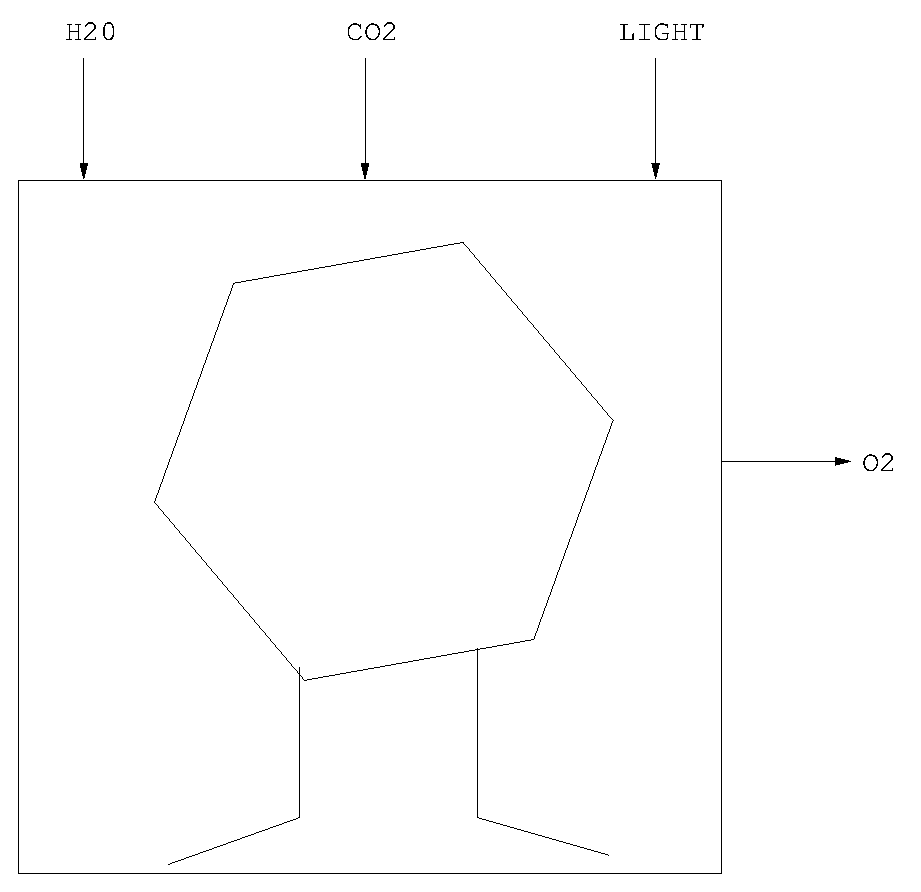
\includegraphics[width=2in]{images/tree.eps}
        \end{figure}
        
      \item[b.] Discuss flow of mass, energy, energy transformations.

        Trees take \ce{CO2}, \ce{H2O} and light from the enviornment. With this, they create the startches and sugars they need to grow. In this case
        energy is taken from the sun and transformed into a energy that can be used by the tree.
    \end{enumerate}

  \item[1.2] A hot cup of tea is placed on a table to cool.
    \begin{enumerate}
      \item[a.] Define a control volume and show energy flows, mass flows, heat transfer, work\dots
        \begin{description}
          \item[Control Volume] It seems a control mass would be more appropriate here as we are looking at the movement of heat and no mass is being added or removed from the tea. For that reason, the system would be defined as the cup and the tea within it.
          \item[Mass Flow] None.
          \item[Heat Transfer] Heat is being transfered from the cup containing the tea to the table.
          \item[Work] No work is being done.
        \end{description}
      \item[b.] Is the system steady or unsteady, open or closed?
        
        Since this is a control mass, it must be a closed system. It is also steady.
    \end{enumerate}

  \item[1.3] A 1000 kg car accelerates from 0 to $100$ km/h in 10 seconds. Determine the work done by the engine, and the power of the engine if,
    \begin{enumerate}
      \item[a.] the road is horizontal. Assuming constant acceleration,
        \begin{align}
         F_N &= m \cdot a \\
         &= 1000kg \cdot 9.8\frac{m}{s} = 9800 N \\
         a &= 2.8\frac{m}{s^2} \\
         d &= \frac{1}{2}a\cdot t^2 \\
           &= 140 m \\
         W &= F \cdot d \\
           &= F_{engine} \cdot d \\
           &= ma \cdot d \\
           &= 2800(140) \\
           &= 3.9 \cdot 10^5 J \\
         P &= \frac{W}{t} \\
           &= 3.9 \cdot 10^{4} W
       \end{align}

       \setcounter{equation}{0}

      \item[b.] the road is on an uphill, with the slope of $5^{\circ}$.
        \begin{align}
         F_{engine} &= mg\cdot sin(\theta) + ma \\
         a &= 2.8\frac{m}{s} \\
         d &= 140m \\
         W &= F_{engine} \cdot d \\
         &= 5.1 \cdot 10^5 J \\
         P &= \frac{W}{t} \\
          &= 5.1 \cdot 10^4 W
        \end{align}

    \end{enumerate}
  \item[1.4] A missle is launched vertically upward from the surface of the earth with an initial velocity of 350 m/s. If the missle is 1200 kg, calculate the maximum height the missle will attain.

    \setcounter{equation}{0}
    \begin{align}
      v &= [350 - 9.8\cdot t]\frac{m}{s} \\
      s &= [350\cdot t - \frac{9.8\cdot t^2}{2}]m \\
      \frac{ds}{dt} &= 350 - 9.8 \cdot t \\
      \frac{ds}{dt} &= 0 \\
      t &= 35.714 s \\
      s |_{t} &= 6250m
    \end{align}

  \item[1.5] A compressed spring exerts $F=100N$ on the top of the piston. The mass of the piston is $M=3kg$, and the diameter is
    $10 cm$.
    \begin{enumerate}
      \item[a.] What is the pressure of the gas in the cylinder, assuming that the outside temperature and pressure are:
        $T=25C$ and $p=1atm$.

        \setcounter{equation}{0}
        \begin{align}
          F_{piston} &= F_{spring} + mg \\
          &= 100N + 29.4N \\
          &= 129.4 N \\
          A &= 0.0025 m^2 \\
          P_{gas} &= \frac{(F_{spring} + mg)N}{A m^2} \cdot \frac{1 atm}{101325\frac{N}{m^2}} + 1atm \\
          &= 1.51 atm
        \end{align}

      \item[b.] Now assume that the temperature of the gas is 100 C. Calculate the pressure of the gas.

        If k is sufficiently large, this becomes a constant volume problem since the change in volume would
        be negligible. The ideal gas law states that temperature is proportional to pressure. In this case,
        temperature increases by a factor of 4, so the pressure must also increase by a factor of 4.

        \setcounter{equation}{0}
        \begin{align}
          P_{new} &= 4 \cdot P_{old} \\
          &= 4 \cdot 1.51 \\
          &= 6.04 atm
        \end{align}

    \end{enumerate}

\end{enumerate}
\end{document}

